\documentclass[11pt]{article}

\usepackage[margin=1in]{geometry}
\usepackage[T1]{fontenc}
\usepackage{lmodern}
\usepackage{microtype}
\usepackage{amsmath,amssymb}
\usepackage{booktabs}
\usepackage{tabularx}
\usepackage{longtable}
\usepackage{array}
\newcolumntype{Y}{>{\raggedright\arraybackslash}X}
\newcolumntype{L}[1]{>{\raggedright\arraybackslash}p{#1}}
\usepackage{graphicx}
\usepackage{xcolor}
\usepackage{tikz}
\usetikzlibrary{positioning,fit,calc,arrows.meta}
\usepackage[font=small,labelfont=bf,skip=6pt]{caption}
\usepackage{float}
\renewcommand{\topfraction}{0.85}
\renewcommand{\textfraction}{0.12}
\renewcommand{\floatpagefraction}{0.75}
\setcounter{topnumber}{3}
\setcounter{totalnumber}{4}
\usepackage{newunicodechar}
\newunicodechar{§}{\S}
\usepackage[numbers,sort&compress]{natbib}
\usepackage[colorlinks=true,linkcolor=blue!50!black,citecolor=blue!50!black,urlcolor=blue!50!black]{hyperref}
\usepackage{cleveref}
\usepackage{enumitem}
\setlist{itemsep=2pt,topsep=4pt}
\usepackage{xurl}
\setlength{\parskip}{0pt}
\renewcommand{\arraystretch}{1.12}

% Writing aids. Set \drafttrue to \draftfalse to hide every note before release.
\newif\ifdraft \drafttrue
\newcommand{\todo}[1]{\ifdraft\textcolor{red}{[TODO: #1]}\fi}
\newcommand{\pending}[1]{\ifdraft\textcolor{orange}{[PENDING #1]}\fi}
\newcommand{\tbd}{\textcolor{orange}{---}}   % empty result cell; never fill with a guess

% Consistent names for the populations and arms.
\newcommand{\edit}{selected edit}

\title{Evaluating Agent-Proposed Weight Edits for False Abstention:\\[2pt]
\large A Controlled Case Study in Qwen2.5-3B-Instruct}
\author{Qamil Mirza\\[2pt]
\small College of Computing, Data Science, and Society, University of California, Berkeley\\
\small\href{mailto:qamilmirza@berkeley.edu}{\texttt{qamilmirza@berkeley.edu}}}
\date{\vspace{-0.6em}Technical report, version 0.3 (draft), \today}

\begin{document}
\maketitle
\vspace{-1.5em}

\begin{abstract}
Small instruction-tuned language models sometimes answer ``unknown'' even when their context contains enough
evidence to answer correctly. In Qwen2.5-3B-Instruct, this false abstention can follow a note in which the model
has already quoted the relevant fact. Earlier interventions recovered correct answers but also encouraged
unsupported answers. We ask whether an agent-proposed weight edit can improve this trade-off.
Following weight-space programming \citep{takehi2026wsp}, a Claude agent inspected the model on an exploration
split and proposed three edits. We evaluated them in a pre-registered case study in one model, with separate
selection and sealed confirmation splits, a transfer split, and six frozen comparators serving repair or pathway
tests. The selected repair was a rank-1 change to the attention output projection in layer 35. It met the
pre-registered repair criterion on sealed data: the base-weighted recovery rate on false abstentions was 82\%,
while unsupported answers on unanswerable questions rose from 3.5\% to 4.2\%. It damaged already-correct answers
at a base-weighted rate of 3\%. Its release-versus-unsupported-answer trade-off was better than a prompt
instruction, activation steering and directional orthogonalisation. The comparison with a simple logit bias
against ``unknown'' was inconclusive. A separate two-head edit provided evidence about a pathway through which
answers can be released, but the agent's explanation of that component was not supported by the pre-registered
tests.

\end{abstract}

\noindent\fbox{\parbox{\dimexpr\linewidth-2\fboxsep-2\fboxrule}{\small
\textbf{Key findings from the sealed evaluation}
\begin{itemize}\setlength\itemsep{1pt}
  \item \textbf{The selected edit met the repair criterion.} The rank-1 edit to the layer-35 attention output
        improved utility by $+0.117$ (95\% CI 0.096 to 0.138). It recovered the correct city on 212 of 261
        false abstentions. Base-weighted unsupported-answer rates rose from 0.035 to 0.042, and damage to
        already-correct answers was 0.030.
  \item \textbf{The comparison with simpler fixes was mixed.} The edit had a better trade-off than an added
        prompt instruction, a layer-29 steering intervention and directional orthogonalisation, after Holm
        correction. Superiority over removing the ``unknown'' option was not established. Against logit bias,
        neither superiority nor equivalence was established.
  \item \textbf{New-city results were consistent with confirmation.} On the descriptive transfer set, utility
        was 0.422 versus 0.303 for the unedited model, recovery was 0.817, and unsupported answers were 0.062
        versus 0.059. This was not a second confirmation test.
  \item \textbf{Repair and explanation were tested separately.} For a different, two-head edit, a layer-33
        intervention was sufficient but not necessary to release answers under the tested conditions.
        The agent's account of what the component computes was not supported by the frozen tests.
\end{itemize}}}
\vspace{0.5em}


\section{Introduction}
\label{sec:intro}

\Cref{fig:example} shows the failure this report studies. The model is given a two-line memory, asked where Ben
lives, and told to write a short note before its answer. The note quotes the relevant memory line, ``Ben lives in
Manchester'', and the answer line then says ``unknown''.

\begin{figure}[t]
\centering\small
\fbox{\begin{minipage}{0.95\linewidth}
\begin{tabular}{@{}l@{\hspace{0.8em}}>{\raggedright\arraybackslash}p{0.76\linewidth}@{}}
\textbf{Memory} & \texttt{user, 2023/03/01 (Wed) 10:00: Ben lives in Manchester.}\\
 & \texttt{user, 2023/03/02 (Thu) 10:00: Ben works as a manager.}\\[3pt]
\textbf{Question} & \texttt{(asked on 2023/03/03 (Fri) 12:00) Where does Ben live?}\\[3pt]
\textbf{Unedited model} & \texttt{Note: user mentioned that Ben lives in Manchester on 2023/03/01 (Wed) 10:00.}\\
 & \texttt{Answer: unknown}\\[3pt]
\textbf{Edited model} & \texttt{Note: user mentioned that Ben lives in Manchester on 2023/03/01 (Wed) 10:00.}\\
 & \texttt{Answer: Manchester}
\end{tabular}
\end{minipage}}
\caption{A false abstention by Qwen2.5-3B-Instruct, copied verbatim from stored outputs (case
\texttt{E-DE01\_ANSa\_H0}). The prompt, given in full in \cref{app:prompt}, ends with ``Note:'', so the
model's output begins with the note. The unedited model quotes the answer
in its note and then abstains. The edited output is the agent's layer-35 edit at dose~1 with the unedited model's
note held fixed (the controlled-prefix setting of \cref{sec:evaluation}). The example comes from the exploration
split, which the agent studied, so it illustrates the failure and is not evidence for the repair.}
\label{fig:example}
\end{figure}

We call this a \emph{false abstention}: the context supports an answer, but the model declines to give one. An
\emph{appropriate abstention} is different, because there the context really does not contain the answer. In this
case study the pattern is common. On the sealed confirmation split, the unedited model abstained falsely on 261
answerable questions, and on 232 of them its note named the correct city, by a frozen matching rule, before the final ``unknown''. The note is
a prompted summary, not a faithful record of the model's computation, so it does not show that the model ``knew''
the answer (\cref{sec:setup}). It does show that the answer was available in the model's own output a few tokens
before the model declined to give it.

\paragraph{Why the failure is hard to fix.}
Recovering these answers is easy if one is willing to make the model answer everything. A useful fix has to release
the missed answers while keeping the model's abstentions on questions that its context cannot answer. Earlier
experiments on the same model and task family (summarised in \cref{sec:background}) found that simple interventions
do not achieve this. Adding a content-free activation direction at layer 29 recovered answers but raised the
unsupported-answer rate on unanswerable questions to 0.188. Removing the ``unknown'' option from the prompt raised it
to 0.451. We therefore score every intervention on both sides of the trade-off: the share of false abstentions it
recovers, and the share of unanswerable questions it answers anyway.

\paragraph{Why evaluate agent-proposed weight edits.}
Recent work shows that a language-model agent can inspect another network and propose a small weight edit that
changes its behaviour \citep{takehi2026wsp}. A weight edit is persistent and cheap to apply. Unlike a prompt change,
it can be inspected and compared directly with other interventions. When the agent is required to state a hypothesis
before it edits, that hypothesis also makes predictions that can be tested. Two risks come with this. An agent that
studies a split of the data can fit that split, and its stated explanation can be wrong even when its edit works.
Evaluating such an edit therefore needs data the agent never saw, a fixed analysis plan, comparison with simpler
interventions, and separate tests for the edit and for the explanation.

\paragraph{What we did.}
A Claude Opus~5.5 agent inspected Qwen2.5-3B-Instruct on an exploration split and submitted three weight edits, each
with a written hypothesis and predictions (\cref{sec:proposals}). We then evaluated the edits in four stages
(\cref{fig:pipeline}). The exploration data screened the submissions; a separate selection split chose a repair
candidate and its dose; the candidates, doses, comparator settings and analysis code were frozen by commit; and only
then were the sealed confirmation and transfer splits generated and read, once each. The evaluation asks two separate
questions. The first is whether an edit repairs false abstention better than five frozen comparators: logit bias, a
prompt instruction, option removal, activation steering and directional orthogonalisation. The second is whether the
agent's proposed pathway and explanation survive intervention tests.

\paragraph{What we found.}
The selected repair is a rank-1 update to the attention output projection of layer 35, the model's last layer. On
sealed data it met the pre-specified repair criterion and had a better recovery-versus-unsupported-answer trade-off
than the prompt instruction, activation steering and orthogonalisation (\cref{sec:results}). It did not clearly
beat the simplest baseline, a logit bias against ``unknown''. That comparison was inconclusive, and removing the
``unknown'' option recovered more answers at a far higher rate of unsupported answers. The edit also broke 3\% of
initially correct answers, which logit bias and steering did not. A different submission, a two-head edit, showed that
changing one layer-33 component is sufficient to release answers. The frozen tests did not establish the agent's
explanation of what that component computes (\cref{sec:explain}).

\paragraph{Contribution.}
The study is a controlled case study with one model, one task family and one agent run. Its contribution is the
evaluation, not the finding that agents can edit weights. We make three points:
\begin{enumerate}[leftmargin=*]
  \item We give an evaluation design for agent-proposed edits that keeps the agent's data, the selection data and
        the confirmation data apart, freezes the analysis before confirmation, and tests repair and explanation
        separately (\cref{sec:evaluation}).
  \item Under that design, an agent-proposed edit repaired false abstention with the evidence in view, and improved
        on three of five simpler interventions under corrected tests. The comparison with logit bias, the simplest
        output-level fix, remains open (\cref{sec:results}).
  \item The edit that worked and the explanation offered for it were separable. A pathway test passed while the
        agent's account of the same component was not established (\cref{sec:explain}).
\end{enumerate}
\Cref{sec:related} places these results in the literature. \Cref{sec:discussion,sec:limits} discuss what they do
not show.

\section{Background and related work}
\label{sec:related}

\subsection{Earlier observations on this model}
\label{sec:background}

This experiment grew out of a project on memory use in small language models.\footnote{Informal write-ups of the
wider project: \href{https://qamil-mirza.com/research/more-than-reasoning}{\emph{More Than Reasoning}} and
\href{https://qamil-mirza.com/research/ai-brain-surgery}{\emph{Weight-Space Programming for Mechanistic
Interpretability}}. This report does not depend on them.}
Four earlier observations motivated it. They come from separate experiments on related controlled tasks and are
context here, not results of this study.
\begin{itemize}[leftmargin=*]
  \item \emph{The behaviour is frequent in this model.} With the evidence in view, Qwen2.5-3B-Instruct abstained on
        0.30 of questions, compared with 0.10 for Llama~3.2~3B, 0.02 for Gemma~3~4B and 0.03 for Phi-4-mini, which
        more often answered wrongly instead. This is a frequency contrast under the tested conditions, not a claim
        that the behaviour is unique to Qwen.
  \item \emph{An answer-related signal is present late.} On failures, the gold answer's first token was among the
        final layer's top-10 tokens in 0.64 of cases for the Qwen model and 0.68 to 0.80 for the three other models.
        On controlled tasks, vocabulary lenses could read out the Qwen answer only in the last six layers. Both are
        readout-dependent observations. They do not show that the answer was derived from the supplied evidence.
  \item \emph{The note usually contains the answer.} In an earlier held-out set, 152 of 165 false abstentions named
        the gold city in the note before ``Answer: unknown''. Asking the model directly whether the memory was
        sufficient did not help: it answered ``no'' on most rows it could answer correctly.
  \item \emph{Ungated pushes are not selective.} A content-free direction added at layer~29, in the style of
        refusal-direction work \citep{arditi2024refusal,lavi2025unanswerability}, recovered answers. So did removing
        the ``unknown'' option. Both increased unsupported answering (to 0.188 and 0.451 respectively). A separate
        gating result reduced this cost, but only on the templates it was built on.
\end{itemize}

\subsection{Related work}

\paragraph{Agents that edit weights.}
Weight-space programming showed that an LLM agent can read a small model's weights and propose an edit; in that work
the agent removed a reasoning-loop direction in Qwen3.5-0.8B by changing 0.016\% of its weights and checked the
result on held-out benchmarks \citep{takehi2026wsp}. Steer2Edit converts steering vectors into edits of individual
heads and neurons \citep{steer2edit2026}. Automated interpretability agents describe components or propose
interventions \citep{shaham2024maia,barez2026agenda}. In a related auditing setting, a calculation tool mattered more
to an LLM's success than access to the weights \citep{liu2026auditors}.

\paragraph{Refusal, abstention and their components.}
Refusal in chat models can be mediated by a single residual-stream direction \citep{arditi2024refusal}, and a linear
direction also tracks unanswerability \citep{lavi2025unanswerability}. Conditional activation steering makes such
interventions input-dependent \citep{lee2025cast}. Individual attention heads can control safety refusal
\citep{zhou2025safetyheads}, and a small set of retrieval heads supports in-context retrieval
\citep{wu2025retrievalheads}. Closest to our failure, a commit-versus-abstain circuit has been described across ten
models from 3B to 14B parameters, and a policy trained on its activations reduced false abstentions
\citep{commitabstain2026}. Abstention can also be a prompt artefact rather than genuine uncertainty
\citep{ling2025artifact}, and answers suppressed by refusal can often be released by local interventions
\citep{liu2026broken}. Behavioural studies document that models misuse sufficient context \citep{joren2025sufficient},
fail to abstain on unanswerable questions \citep{kirichenko2025abstentionbench}, and use internal confidence to
decide whether to abstain \citep{kumaran2026confidence}.

\paragraph{Selective interventions.}
Selectivity is an established concern. False-refusal vector ablation removes a direction from the weights and scores
released false refusals against preserved true refusals \citep{wang2025falserefusal}. Residual Paving adds trained
gated residual modules to a frozen backbone and scores a change in the target behaviour against preserved benign
behaviour and wanted refusals \citep{hinkley2026paving}. SAE-feature steering can trade answering against abstention
\citep{hasanov2026drno}. These studies concern safety refusal or use activation-level methods; none is agent-proposed.

\paragraph{Pre-registration in interpretability.}
Pre-registered, once-only held-out tests have been used for representation steering outside language models
\citep{readablenotsteerable2026}. Knowledge-editing methods such as ROME and MEMIT \citep{meng2022rome,meng2023memit}
edit stored facts. Our target is a decision behaviour, not a stored fact. \Cref{app:related} compares each study
with ours.

\subsection{What this study adds}
\label{sec:new}

Each part of this study has precedent: agent-proposed weight edits, selective refusal interventions,
component-level accounts of abstention and pre-registered interpretability tests. What we add is their combination
in one evaluation:
\begin{itemize}[leftmargin=*]
  \item false abstention with sufficient evidence in the context, not safety refusal or closed-book uncertainty;
  \item an edit proposed by an agent that could see only an exploration split;
  \item outcome measures for both sides of the trade-off (answers recovered, unsupported answers, damage to correct
        answers, and following changed evidence);
  \item one confirmatory read of sealed data, with candidates, doses and analysis frozen beforehand; and
  \item frozen comparisons with prompt, steering, orthogonalisation and logit-bias interventions, and separate
        tests of the agent's mechanistic account.
\end{itemize}
We are not aware of an earlier pre-registered test on sealed data of an agent-proposed weight edit for false
abstention with the evidence in view. This rests on a targeted search, not a systematic review. We also found no
earlier head-to-head comparison of a weight edit with a logit bias for abstention. Our results leave that comparison
open (\cref{sec:results}).

\paragraph{What pre-registration means here.}
The protocol was not lodged with an external registry. Pre-registration here means that each design stage was
committed to the project's Git repository, with hashes, before the data it governed were generated. The analysis
code and selected settings were committed (freeze F2, \cref{sec:evaluation}) before any confirmation output existed.
Readers can check this order in the commit history once the repository is public (\cref{app:artefacts}).

\section{The experimental setup}
\label{sec:setup}

We evaluated Qwen2.5-3B-Instruct, a 36-layer model, in fp32 with greedy decoding. The prompt asks it to write
a short memory note and then an \texttt{Answer:} line containing a city or ``unknown''. The instruction
explicitly offers ``unknown'' when the memory does not supply an answer.

\paragraph{What the note tells us.}
The note is a prompted summary of the memory, not a verified reasoning trace. When we describe a response as
``note, then refuse'', we mean that the gold city appears in that summary before \texttt{Answer: unknown}.
This shows that the city was written down. It does not establish that the model completed an internal
derivation, and we do not treat the note as a faithful explanation of the computation.

\paragraph{Tasks and examples.}
The synthetic memories support three tasks: \textbf{direct extraction (DE)}, such as ``Where does A live?'';
\textbf{relational composition (RC)}, such as ``In which city does A's supervisor work?''; and
\textbf{temporal updating (TU)}, such as ``Where does A live now?'' after a move.
Each underlying \emph{base case} produces 13 related rows: 6 answerable rows (two variants at three hardness
levels), 3 unanswerable rows with a related distractor (UNA-rel), 1 unanswerable row with a swapped name
(UNA-swap), and 3 counterfactual rows in which the evidence specifies a different city (CF).

We call the unedited model \textbf{B0}. Its responses define the populations used throughout the evaluation:
\textbf{FA} contains answerable rows on which B0 abstains falsely; \textbf{C} contains answerable rows it gets
correct; \textbf{UNA} contains all unanswerable rows; and \textbf{CF} contains the changed-evidence rows.
Each intervention is evaluated on the same fixed populations.

\paragraph{Splits.}
Related variants stay together when cases are assigned to exploration, selection, confirmation and transfer
splits (\cref{tab:splits}). The partition also prevents a person--evidence-city key, including a
counterfactual variant's key, from crossing splits. No canonical base key or exact memory text appears in two
splits. Names, cities and templates can still be shared; disjoint cases do not imply entirely different
vocabularies. The agent saw only the exploration split, E.

\begin{table}[ht]
\centering\small
\begin{tabularx}{\linewidth}{@{}llYY@{}}
\toprule
Split & Bases per task & Access & Purpose \\
\midrule
E & 48 & Agent & Exploration only \\
S & 32 & Analysts & Dose selection and candidate selection \\
H & 48 & Sealed; read once & Confirmation \\
T-city & 24 & Sealed; read once & Transfer to new cities \\
\bottomrule
\end{tabularx}
\caption{E and S use generator seed 51 with disjoint cases, H uses seed 52, and T-city uses seed 53.
Rows from earlier experiments are excluded by prompt hash. A second planned transfer split with a reworded
instruction, T-format, was dropped before the first design freeze (F0).}
\label{tab:splits}
\end{table}

\paragraph{Scoring.}
A frozen rule-based grader scores the answer after the last \texttt{Answer:} marker, separately from the note
(\cref{app:methods}). It distinguishes a correct answer, abstention, wrong answer, mixed answer and abstention,
conflicting answers, other content, and degenerate or missing outputs.

The primary utility, $U$, rewards a correct answer with $+1$ and assigns abstention $0$. A mixed answer receives
$0$ on an answerable row and $-1$ on an unanswerable row; other errors receive $-1$. Within each base,
answerable and unanswerable rows each contribute half the weight. Counterfactual rows are scored separately
and do not enter $U$. We also report:
\begin{itemize}
  \item \textbf{Recovery (Rel):} the share of baseline false abstentions that become correct answers.
  \item \textbf{Unsupported answering (Uns):} the share of unanswerable rows given an asserted or suggested answer.
  \item \textbf{Damage (Dam):} the share of baseline-correct rows that are no longer correct.
  \item \textbf{Counterfactual following (CF-follow):} the share of changed-evidence rows answered with the new city.
  \item \textbf{Degenerate outputs (Deg):} degenerate responses and responses missing an answer marker.
\end{itemize}
Rates are base-weighted. We also give raw row counts where useful; these need not yield the same percentages.

\paragraph{Comparators.}
Five interventions serve as repair baselines, with settings frozen after selection on S:
\begin{itemize}
  \item \textbf{B1, logit bias:} penalise ``unknown'' tokens after the answer marker.
  \item \textbf{B2, added instruction:} append ``Do not reply unknown.'' to the prompt.
  \item \textbf{B3, option removal:} remove the ``unknown'' option from the instruction.
  \item \textbf{B4, activation steering:} apply the earlier refusal-direction push at layer 29.
  \item \textbf{B5, directional orthogonalisation:} remove a direction fitted on E from the relevant weights,
        following an adaptation of \citet{arditi2024refusal}.
\end{itemize}
A sixth comparator, \textbf{B6}, consists of five size-matched random edits. It is used in the pathway tests,
not in the main repair comparison (\cref{sec:explain}).

\begin{figure}[ht]
\centering
\begin{tabularx}{\linewidth}{@{}YYYY@{}}
\toprule
\textbf{Explore} & \textbf{Select} & \textbf{Freeze} & \textbf{Evaluate} \\
\midrule
Agent proposes edits on E; the harness replays them. &
S selects candidates and doses separately for repair and pathway tests. &
F2 fixes candidates, settings and analysis before confirmation. &
H tests the frozen claims; T-city checks transfer descriptively. \\
\bottomrule
\end{tabularx}
\caption{The agent sees only E. S selects the candidates and doses for repair and pathway tests. The
confirmatory plan is frozen by commit before any model outputs on H or T are generated; each is then read once.}
\label{fig:pipeline}
\end{figure}

\section{What the agent proposed}
\label{sec:proposals}

\paragraph{The agent and its sandbox.}
The editor was a fresh Claude Opus~5.5 session, run through the API. It had read-only access to the exploration
split E and no access to the project's records or to S, H or T-city. Its tools could run the model, record
activations, apply candidate edits and run Python. Analysis was limited to closed-form operations such as means,
covariances, projections, SVD and single linear solves. Gradients, optimisers and iterative loss-based fitting were
not allowed.

\paragraph{What an edit could change.}
An edit could change at most four components, where a component is the attention output projection
(\texttt{o\_proj}), the MLP output projection (\texttt{down\_proj}) or one of the two layer norms of a given layer.
Within a component the edit was either a dense update of rank at most 4 or a sparse edit of whole rows or columns
(at most 512 per candidate). The query, key, value, gate and up projections, the embedding, the unembedding, the
final norm and the rows for ``unknown'' tokens were off limits. Before testing an edit, the agent had to name the
component, state what it believed the component computes, predict outcomes for each row type and predict activity
in the unedited model. Each submission also fixed a primary outcome (its \emph{signed endpoint}), a most important
component and a scalar variable $f$ that its account says the component computes.

\paragraph{The run.}
The run took 73 turns, 16 model-pass requests and 63 Python runs, and saved six edits, of which the agent submitted
three. It lasted about 9.7 hours from start to the last submission, and its API cost was \$3.58.
\Cref{tab:submissions} summarises the submissions. The hypotheses are the agent's claims, recorded before any
evaluation; they are not established explanations.

\begin{table}[t]
\centering\small
\caption{The agent's three submissions. The hypotheses are abridged from the stored submission records; quoted
phrases are verbatim. ``Weights changed'' counts matrix entries altered by the edit.}
\label{tab:submissions}
\begin{tabularx}{\linewidth}{@{}lL{0.25\linewidth}Y@{}}
\toprule
\# & Edit & The agent's hypothesis (a claim, not an established explanation) \\
\midrule
1 & Zero the \texttt{o\_proj} columns of heads L32h2 and L33h10. Repair; about 0.52M weights changed. &
The two heads write ``a nearly constant `unknown' vector'' at the answer position, the same in every population.
This ``acts as an evidence-independent default-abstention prior''. Other late heads write the evidence city, more
strongly when the evidence is clearer. False abstention occurs when the city signal is only moderately weak, so the
prior wins. Removing the prior should recover false abstentions but not change unanswerable rows, where the
``unknown'' margin is much larger. \\
\addlinespace
2 & Rank-1 update of the layer-35 \texttt{o\_proj}. Repair; about 4.19M weights changed, from two 2048-dimensional
vectors. &
Layer-35 attention ``carries an `an answer is available in the memory/note' signal'' at the answer position,
almost as strong on false abstentions as on correct answers and absent on unanswerable rows. The model does not turn
this signal into suppressing ``unknown''. The edit reads the signal and writes it toward city tokens and away from
``unknown''. Because it sits in the last layer, ``it cannot be undone by self-repair''. \\
\addlinespace
3 & Double the same two heads' \texttt{o\_proj} columns. Diagnostic; about 0.52M weights changed. &
The converse of edit 1. If the heads supply the abstention prior, strengthening them should turn correct answers
into ``unknown'' while the note still names the city. \\
\bottomrule
\end{tabularx}
\end{table}

\paragraph{The selected repair in detail.}
Edit 2 adds a rank-1 matrix to the layer-35 output projection $W_O \in \mathbb{R}^{2048 \times 2048}$:
\[
  W_O \;\leftarrow\; W_O + s \, c \, d\,(W_O^{\top} w)^{\top}.
\]
Here $w$ is a read direction found by one closed-form solve on E. It was chosen to be large on answerable rows and
small on unanswerable rows. The write direction $d$ is a unit vector that the agent built from the difference between the
mean city unembedding and the ``unknown'' unembedding. The constant $c = 20$ is the agent's scale, and $s$ is the dose chosen on S. For an attention output
$a$, the edit adds $s\,c\,(w^{\top} W_O a)\,d$ to the residual stream: it reads the projection of the original
layer output onto $w$ and writes that amount along $d$. The update has rank 1 and is stored as two vectors. Its
dense matrix still changes almost every entry of $W_O$, which is why we describe it as a low-rank update and not as
a sparse one.

\paragraph{The agent's predictions.}
For edit 1, the agent predicted recovery of about 85\% of false abstentions, at least 97\% of correct answers
retained, and an increase in unsupported answers on related-distractor rows from about 1\% to at most 4\%. For
edit 2, it predicted 75--80\% recovery, 92--97\% of correct answers retained, and unsupported answering on those rows
staying at or below 3\%. For edit 3, it predicted that 30--40\% of correct answers would become ``unknown''. These
predictions were recorded for later scoring. They did not influence selection.

\section{The independent evaluation}
\label{sec:evaluation}

The evaluation separates two questions: whether an edit \emph{repairs} false abstention (branch R), and whether
the proposed \emph{pathway and explanation} survive intervention tests (branch M). Each branch can select a
different edit and dose. Success in one does not imply success in the other.

\paragraph{Replay and screening on E.}
After the agent finished, the evaluation harness replayed every submission on all of E. The repair screen
required a utility gain over B0 with a one-sided 97.5\% lower bound above zero and at least 20 false-abstention
bases in DE or RC. The pathway screen required an effect of at least 0.05 in the declared direction, with a
one-sided 97.5\% bound beyond zero and at least 20 bases in the relevant endpoint population. If no submission
met either screen, S, H and T would have remained unread. E outcomes remained exploratory because the agent
had used that split to develop the edits.

\paragraph{Selection on S.}
The entry rules were then evaluated on S. For repair, candidate and comparator doses were chosen to maximise
utility, and the qualifying candidate with the highest utility was selected; candidate ties favoured fewer
edited weights. For the pathway branch, dose selection maximised the declared signed effect, subject to the
pre-registered limit on degenerate outputs. Candidate selection used the standardised effect, separately from
repair. Dose ties favoured the setting closest to no change.

The repair candidate was submission 2, a rank-1 edit to the layer-35 attention output projection, at dose 2.
Its utility on S was 0.429, compared with 0.402 for the next submission and 0.303 for B0. Dose 2 was the top of
the frozen grid; larger doses were not searched. The pathway candidate was submission 1, the two-head edit,
at dose 1.5, with the layer-33 head designated as its primary component. Selected repair-comparator doses
were $-8$ for logit bias (B1), 1 for steering (B4), and $\beta = 1$ for orthogonalisation (B5).

\paragraph{Freezing the confirmation.}
The selected candidates, doses, comparator settings and analysis code were frozen before any H or T model
outputs were generated or read. This freeze, F2, is recorded at commit \texttt{02bb2f6}, with design hash
\texttt{d02d9f9c\ldots}. The confirmation run checked that commit before accessing H or T.

\paragraph{Decision criteria.}
H and T were each evaluated once. The repair criterion on H required a positive lower bound for the utility
gain, damage no greater than 0.05, degenerate outputs no greater than 0.02, and counterfactual following of at
least 0.90. The damage and counterfactual thresholds applied to point estimates; uncertainty was reported
alongside them.

A better trade-off than a repair comparator could be established in either of two ways:
\textbf{O1}, higher recovery with an unsupported-answer increase smaller than 0.05; or
\textbf{O2}, fewer unsupported answers with a recovery loss smaller than 0.05. Superiority and non-inferiority
had to pass together for the relevant orientation. Holm correction covered all ten comparisons---two
orientations for each of B1--B5. Pathway tests formed a separate family (\cref{sec:explain}).

\paragraph{Uncertainty.}
We used a paired bootstrap clustered by base and stratified by task, with $B = 10{,}000$ draws.
Intervals are 95\% unless stated otherwise. The intervals describe uncertainty in individual estimates;
confirmatory decisions use the corrected tests. \Cref{app:methods} gives the inference rules.

\section{Results}
\label{sec:results}

All results in this section come from the sealed confirmation split H (144 base cases, 1,872 rows), except the
transfer check at the end. H contains 261 false abstentions, 593 baseline-correct rows and 576 unanswerable rows.

\subsection{The selected edit meets the repair criterion}

The rank-1 layer-35 edit met all four pre-specified conditions. Utility rose from 0.317 to 0.435, a gain of
$+0.117$ (95\% CI 0.096 to 0.138). The edit gave the gold city on 212 of the 261 false abstentions, a base-weighted
recovery of 0.816. Unsupported answers rose from 20 to 24 of 576 unanswerable rows (0.035 to 0.042). Damage was
0.030, below the 0.05 limit on the point estimate, although its upper confidence bound was 0.055. Degenerate
outputs were 0.008 (limit 0.02), and counterfactual following was 0.917, against a threshold of 0.90 and 0.632 for
the unedited model.

The repair has a visible cost. The edit broke 11 of 593 previously correct answers (base-weighted damage 0.030).
Logit bias (B1) and layer-29 steering (B4) broke none of them.

\subsection{Comparison with simpler interventions}

\Cref{tab:h} gives every arm's rates and the outcome of each trade-off test, and \cref{fig:tradeoff} plots recovery
against unsupported answering. The edit's trade-off was better than that of the added instruction (B2, via O2,
Holm-adjusted $p = 0.005$), activation steering (B4, O2, $p = 0.033$) and directional orthogonalisation (B5, O1,
$p = 0.007$). Against B2 and B4 the edit gave fewer unsupported answers without losing recovery; against B5 it
recovered more without adding unsupported answers.

\begin{table}[t]
\centering\small
\caption{Sealed confirmation results on H. Rates are base-weighted means (\cref{sec:setup}); $U$ is utility with
error penalty 1. The last column reports whether the selected edit's trade-off is better than that comparator's, with
the orientation that passed and its Holm-adjusted $p$-value across ten tests. Values were recounted independently
from per-row outputs.}
\label{tab:h}
\setlength{\tabcolsep}{5pt}
\begin{tabularx}{\linewidth}{@{}Yrrrrrl@{}}
\toprule
 & \multicolumn{1}{c}{Recovery} & \multicolumn{1}{c}{Unsupp.} & \multicolumn{1}{c}{Damage} &
 \multicolumn{1}{c}{CF-follow} & \multicolumn{1}{c}{$U$} & Edit better? \\
 & \multicolumn{1}{c}{$\uparrow$} & \multicolumn{1}{c}{$\downarrow$} & \multicolumn{1}{c}{$\downarrow$} &
 \multicolumn{1}{c}{$\uparrow$} & \multicolumn{1}{c}{$\uparrow$} & (test, $p_{\mathrm{Holm}}$) \\
\midrule
B0 unedited & 0 & 0.035 & 0 & 0.632 & 0.317 & --- \\
\textbf{Selected edit} (rank-1, L35, dose 2) & \textbf{0.816} & \textbf{0.042} & \textbf{0.030} & \textbf{0.917} &
  \textbf{0.435} & --- \\
\midrule
B1 logit bias ($-8$) & 0.793 & 0.095 & 0 & 0.919 & 0.406 & inconclusive \\
B2 ``Do not reply unknown'' & 0.721 & 0.083 & 0.046 & 0.882 & 0.389 & yes (O2, 0.005) \\
B3 ``unknown'' option removed & 0.977 & 0.682 & 0.021 & 0.975 & 0.130 & not established \\
B4 layer-29 steering ($\alpha = 1$) & 0.786 & 0.078 & 0 & 0.921 & 0.418 & yes (O2, 0.033) \\
B5 orthogonalisation ($\beta = 1$) & 0.678 & 0.031 & 0.099 & 0.838 & 0.401 & yes (O1, 0.007) \\
\bottomrule
\end{tabularx}
\end{table}

\begin{figure}[t]
\centering
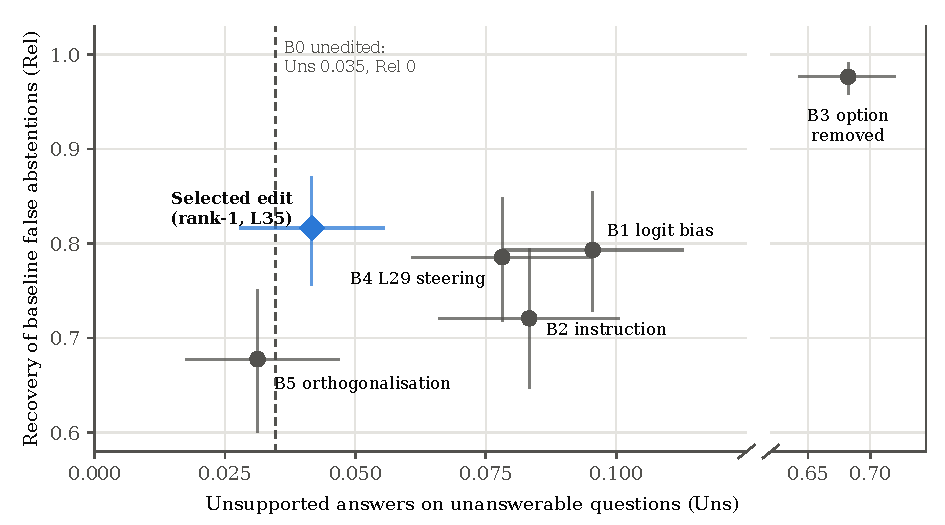
\includegraphics[width=\linewidth]{figures/fig2-tradeoff.pdf}
\caption{Recovery against unsupported answering on H for the selected edit and the five repair comparators. Up and to
the left is better. Bars are marginal 95\% bootstrap intervals for each rate, computed after confirmation from the
stored per-row outputs (\cref{app:figdata}). They are descriptive. The confirmatory comparisons in \cref{tab:h} use
paired differences and Holm correction, so overlapping marginal intervals do not imply that a comparison failed, and
separated ones do not imply that it passed. The dashed line marks the unedited model's unsupported-answer rate; its
recovery is 0 by definition. The horizontal axis is broken to show B3.}
\label{fig:tradeoff}
\end{figure}

\paragraph{Logit bias: inconclusive.}
The comparison with B1 is the most informative result in the study, because B1 is the simplest intervention that
targets the output directly. The point estimates favour the edit: recovery 0.816 against 0.793, and unsupported
answers 0.042 against 0.095. The difference in unsupported answers is clear (edit minus B1: $-0.054$, 95\% CI
$-0.069$ to $-0.038$). The difference in recovery is not ($+0.023$, 95\% CI $-0.043$ to $+0.088$). O2 therefore
depends on whether the edit's recovery is at most 0.05 below B1's. That non-inferiority component gave $p = 0.015$,
which did not survive Holm correction (adjusted $p = 0.092$). Equivalence was not shown either: TOST gave $p = 0.21$
for recovery and $0.70$ for unsupported answering. The data do not show that the edit is better than logit bias, and
they do not show that the two are equivalent. B1 also has an advantage the trade-off tests do not score: it broke no
previously correct answers.

\paragraph{Option removal: not established.}
Removing the ``unknown'' option (B3) recovered almost every false abstention (0.977), but it answered 0.682 of
unanswerable questions. The edit recovered less ($-0.160$) and gave far fewer unsupported answers ($-0.641$). Neither
orientation passes: O1 fails because the edit recovers less, and O2 fails because the recovery loss exceeds the 0.05
margin. The frozen tests cannot rank two arms that sit at such different points of the trade-off. On utility, which
weighs both sides equally, B3 scored 0.130 against the edit's 0.435, but utility was not a pre-specified comparison
between arms.

\paragraph{False abstentions whose note names the city.}
In 232 of the 261 false abstentions on H, the unedited model's note names the gold city (by the frozen
answer-bearing rule). On this subset, the edit and B1 recovered at similar rates (0.864 and 0.881). This comparison
is descriptive and was not tested.

\subsection{Transfer to unseen cities}

T-city has 24 bases per task and uses cities that appear in no other split. It was read once and is a descriptive
check, not a second confirmation. The results resemble those on H. Utility was 0.422 against 0.303 for the unedited
model, recovery 0.817, unsupported answering 0.062 against 0.059, damage 0.031 and counterfactual following 0.912.
Comparator utilities fell in the same order as on H: B4 0.415, B1 0.412, B5 0.409, B2 0.397, B3 0.107. T-city
changes only the answer vocabulary. It does not test new tasks or reworded instructions.

The edit's selection-split results were also close to its confirmation results (utility 0.429 on S and 0.435 on H;
counterfactual following 0.910 and 0.917). We report this consistency as description, not as extra evidence, because
S was used to select the edit.

\section{What the edits explain}
\label{sec:explain}

An edit can improve answers without explaining why the original model failed. We therefore distinguish
\emph{repair}, a beneficial change in behaviour; \emph{pathway evidence}, an intervention linking the edit's
effect to a named component; and a \emph{mechanistic account}, a description that also predicts the unedited
model's behaviour. The repair result above concerns the layer-35 edit. The pathway evaluation selected a
different candidate: the two-head edit, at dose 1.5, with the layer-33 head fixed in advance as the primary
component.

\paragraph{A pathway through layer 33.}
Both pathway tests passed after Holm correction across the three branch-M tests ($p < 0.001$).
Reverting the layer-33 component in the edited model reduced recovery on false abstentions by 0.293
(95\% CI 0.225 to 0.368). The edit also recovered 0.717 more than the mean of five size-matched random edits,
B6. These tests address the effect of changing that component and the comparison with random perturbations.

Two activation interventions asked whether the effect could be transferred or blocked. Adding the edit's
change to the layer-33 output at the answer position in the unedited model recovered 0.808 of false
abstentions. Clamping that output back to its original value in the edited model removed only 0.193.
The layer-33 intervention was therefore sufficient, but not necessary, to release answers under these
conditions. The remaining recovery is consistent with another route, possibly through the layer-32 head;
that explanation was not directly tested. Without a random-head comparison, these results do not establish
that the two selected heads have a unique role.

\paragraph{The explanation was not established.}
The agent's account of what the component computes was not supported by the frozen tests. Its proposed
variable added no predictive value for false abstention, although the baseline predictor already had an
AUROC of 0.998 and left little room for improvement. Intervening on the variable also failed to establish a
different effect on answerable versus unanswerable questions relative to a matched logit bias: the
interaction was 0.0005 (95\% CI $-0.025$ to 0.027). Two activity predictions held, but the combined account
test did not pass.

This negative has an important qualification. The agent described the heads as an evidence-independent
``unknown'' prior. A null interaction is close to what that description would predict, so the frozen predictor
and interaction tests fit this account poorly. The result means that the account was not shown by the
pre-registered tests; it is not a refutation of that account.

At its pathway-test dose, the two-head edit was also not selective: on S it produced unsupported answers on
96\% of unanswerable rows. The pathway result identifies where an answer-release effect can be produced.
It does not explain the selected layer-35 repair.

\paragraph{Exploratory observations.}
On E, doubling the two heads changed 180 of 572 correct answers (31\%) into ``unknown'', within the agent's
prediction of 30--40\%. Removing the heads recovered most false abstentions on that split. These observations
motivated the bidirectional interpretation, but E was the split the agent studied and cannot independently
confirm it. The exploratory results are collected in \cref{app:e}.

\section{Discussion}
\label{sec:discussion}

\paragraph{What the repair establishes.}
Under a design that kept the agent away from the selection and confirmation data, an agent-proposed weight edit
improved this model's handling of false abstention on unseen cases. It met a criterion fixed in advance, and it did
better than three of five simpler interventions under corrected tests. The result is an existence proof under
controlled conditions. It shows that a closed-form, agent-designed rank-1 edit can move this model to a better point
on the recovery--unsupported-answer trade-off than several standard fixes. It does not show that agent-proposed edits
generally do so, or that this edit is the best of its kind.

\paragraph{Why the logit-bias comparison matters.}
A logit bias against ``unknown'' changes nothing inside the model; it only makes one answer less likely at the
output. If an internal edit cannot clearly beat it, the edit's benefit may amount to an output-level shift that
happens to be implemented in the weights. Our data leave this open. The edit gave clearly fewer unsupported answers
than B1 at similar recovery, but the test could not rule out a recovery deficit larger than the 0.05 margin after
correction, and B1 broke no correct answers while the edit broke 3\%. A larger confirmation set, or a comparison
targeted at B1 alone, would be needed to resolve it.

\paragraph{Is there an edit-specific mechanism?}
The evidence does not yet show one. The layer-35 edit was selected and confirmed on behaviour. Its own explanation,
an ``answer available'' signal read by the edit, was not tested in the confirmation; the pathway branch tested the
other submission. Whether the edit's read direction matters, as opposed to its write direction toward cities, is the
first question of the follow-up below.

\paragraph{Improving behaviour is not the same as explaining it.}
The study separated the two on purpose, and they came apart. The agent's two-head edit located a component that is
sufficient to release answers, yet the account the agent gave of that component was not established. The agent's
predictions were often numerically close (31\% of correct answers flipped to ``unknown'' on E, inside its predicted
30--40\%), but close predictions on the agent's own data are weak evidence for an account. A useful edit and a
plausible story can both be produced without the story being right. Evaluations of agent-proposed interventions
should test the two separately.

\paragraph{One model and synthetic tasks.}
Every confirmatory result concerns one 3B model on generated city questions with a fixed instruction and note
format. The false-abstention behaviour itself was much rarer in the three other small models we had examined
(\cref{sec:background}), so the problem this edit solves may be specific to this model and prompt. The T-city check
varies only the answer vocabulary. Natural questions, reworded instructions and misleading contexts
\citep{setiawan2026grabrag} remain untested.

\paragraph{The dose grid.}
The selected dose was the top of its frozen grid, and utility on S was still rising there. The orthogonalisation
comparator was also selected at the top of its grid ($\beta = 1$). A wider grid could change the comparison in either
direction: a larger edit dose might recover more but also break more correct answers. The edit should be read as one
point on a dose curve that was not fully explored.

\paragraph{One agent run.}
The study observed one session of one agent. Another session, another prompt or another model could propose different
edits, better or worse. We did not test whether access to weights was necessary for the agent's success; in a related
auditing setting, a calculation tool mattered more than weight access \citep{liu2026auditors}. Estimating how often
agents produce edits that pass this evaluation would require many runs.

\paragraph{Controls still needed.}
Three controls would sharpen the conclusions: random-head and random-direction controls, to test whether the chosen
components and directions are special; natural-question data with the evidence in view; and comparisons with
component-level methods such as Steer2Edit \citep{steer2edit2026}, weight-folded false-refusal ablation
\citep{wang2025falserefusal}, gated refusal edits \citep{hinkley2026paving} and SAE-feature steering
\citep{hasanov2026drno}. Our comparisons do not establish superiority over editing or steering methods in general.

\subsection{Pre-registered follow-up (in progress; no results reported)}
\label{sec:followup}

A follow-up was pre-registered after the confirmation closed, to ask whether the two edits are specific. It uses a new
controlled split, N (seed 54, 1,950 rows), disjoint from the agent's exploration split and the selection split, and
it cannot change any confirmation verdict above. Its design and manifest were committed before any held-out output
was generated (\cref{app:artefacts}). \textbf{No follow-up results exist at the time of writing, and none are
reported here.}

\begin{itemize}[leftmargin=*]
  \item \emph{Does the layer-35 read direction matter (C4)?} Twenty control edits keep the edit's write vector but use
        a random read vector. Each is scaled on development rows to match the edit's root-mean-square gate and is
        sign-aligned to push in the same direction. C4 passes if the edit's utility exceeds all twenty controls and its
        unsupported-answer rate is below their median. A failure would leave read-side specificity unestablished; on
        its own it would not show equivalence to an output bias.
  \item \emph{Are the two heads unusual (C1, C2)?} C1 requires ablating the target pair to recover more false
        abstentions than each of twenty random pairs from the same layers, by at least 0.30 over their median. C2
        requires doubling the target pair to create more abstentions on previously correct rows than doubling each
        random pair.
  \item \emph{Does the layer-35 signal follow the agent's predictions (C5)?} Four frozen predictions concern how the
        proposed signal changes when evidence is removed, the city changes, distractors are added, or unrelated
        evidence replaces absent evidence.
\end{itemize}
C1, C2 and C4 require an empirical rank of 1 among 21 evaluated edits; C5 uses an intersection--union test at 0.05.
No family-wise error control is claimed. Under a null in which the target's scores are exchangeable with the random
controls' (ties counted against the target), and given a valid C5 test, a union bound puts the chance of at least one
false pass at about 0.19 or less. This bound holds only under that null; it is not a guarantee against every possible
mechanism. Descriptive arms examine single heads, other late-layer pairs, random write vectors, direct logit
attribution and the prompt without its ``unknown'' option. A natural-question check uses 138 LongMemEval development
questions with the evidence in view.

\section{Limitations, reproducibility and resources}
\label{sec:limits}

\paragraph{Main limitations.}
\begin{itemize}[leftmargin=*]
  \item \emph{Scope.} One model (Qwen2.5-3B-Instruct), synthetic city questions in three task templates, one
        instruction and note format, and one agent run. The planned reworded-instruction split was dropped before the
        first freeze, so transfer to new instructions is untested.
  \item \emph{Unresolved comparison.} The comparison with logit bias is inconclusive (recovery difference 95\% CI
        $-0.043$ to $+0.088$); neither superiority nor equivalence was established at the frozen margins.
  \item \emph{Costs of the repair.} The edit broke previously correct answers (base-weighted damage 0.030, upper bound
        0.055), while B1 and B4 broke none. Counterfactual following (0.917) cleared its 0.90 threshold by a small
        margin. Both thresholds were applied to point estimates.
  \item \emph{Dose.} The selected dose was the largest in the frozen grid, and larger doses were not searched.
  \item \emph{Controls.} The only random-edit control in confirmation was B6, five size-matched perturbations of the
        same weight entries, used in the pathway tests. Random-head and random-direction controls belong to the
        follow-up. The prompt offers ``unknown'', and the present results do not distinguish a change in how the
        model treats that option from a change in how it uses the evidence.
  \item \emph{Mechanism tests.} The account test faced a predictor ceiling (baseline AUROC 0.998) and fitted the
        agent's account poorly (\cref{sec:explain}). The pathway result is sufficiency, not necessity.
  \item \emph{The note.} The note is a prompted summary. We do not treat it as a faithful trace of the model's
        reasoning.
\end{itemize}

\paragraph{Reproducibility.}
The design was frozen in three stages before the data each stage governed were generated: F0 (data, grader,
comparators, edit rules), F1 (bounds, run procedure, cost limits) and F2 (candidates, doses, analysis code). All
model outputs on H and T-city were generated after F2. Besides two deviations recorded at F1, four tooling fixes
were made: a comparator file missing from the run bundles, smoke tests that could not apply full-size edits, a
missing key that crashed the first selection run (\$0.09, counted in the cost below), and a guard failure that
exited without a log message. None changed a scoring, selection or decision rule, and each was reviewed and accepted
in the project record. \Cref{app:artefacts} lists the commits, hashes, code and per-row outputs, and states which
artefacts are not yet public.

\paragraph{Compute and cost.}
The agent run cost \$3.58 in API usage. Replaying the submissions on E took about 59 hours on a laptop CPU at no
cloud cost. Selection on S ran on one NVIDIA A40 GPU and cost \$4.38, including \$0.09 for a failed first attempt;
confirmation on H and T-city took 4.36 hours on one A40 and cost \$2.57. Total GPU charges were \$6.95.

\section{Conclusion}
\label{sec:conclusion}

This case study asked whether an AI agent can propose a weight edit that repairs a specific failure, Qwen2.5-3B
answering ``unknown'' with the answer in its own note, without teaching the model to answer what it cannot support.
Under an evaluation that kept the agent's data, the selection data and the confirmation data apart, the answer for
this model and task is yes. A rank-1 edit to the last attention layer recovered most false abstentions on sealed
data, added few unsupported answers, and beat three of five simpler fixes on pre-specified trade-off tests. It broke
a small share of correct answers, and it did not clearly beat a logit bias against ``unknown''.

The study does not show that the agent understood why the model fails. The component it named for a different edit
lies on a route that can release answers, but the agent's account of that component was not established, and the
selected repair's own explanation was not tested. The natural next question is whether the edit is specific: whether
its read direction and the agent's chosen heads matter, and whether its advantage over output-level fixes survives
natural questions and other models. The pre-registered follow-up in \cref{sec:followup} addresses the first part of
that question.


\section*{Disclosure of AI assistance}
The weight edits studied here were proposed by Claude Opus~5.5 (Anthropic), run through the API as the agent
described in \cref{sec:proposals}. AI assistants (Claude and GPT models) also helped design the study, write and
review the analysis code, independently recount the results from per-row outputs, and draft and edit this report.
The author reviewed the design, the results and the text, and is responsible for the content.
\todo{Author to confirm this wording, in particular the final sentence.}


\ifdraft
% Shown only in draft builds (\drafttrue in main.tex). Keep in step with EDITORIAL_REVIEW.md.
\section*{Unresolved before publication (draft only)}
\begin{enumerate}[leftmargin=*]
  \item \textbf{Public artefacts.} No public repository URL or archive DOI yet; the pre-registration order can only be
        checked by readers once the commit history is public (\cref{app:artefacts}).
  \item \textbf{Edited weights and transcript.} Confirm the model licence permits releasing edited weights; confirm the
        redacted agent transcript is ready to publish.
  \item \textbf{Disclosure wording.} Author to approve the AI-assistance statement.
  \item \textbf{Follow-up.} \Cref{sec:followup} has no results. Either keep it as a labelled in-progress section or
        remove it before release; do not add results until the follow-up is recounted and reviewed.
  \item \textbf{Bibliography caveats.} Kumaran et al.: journal version not confirmed from a primary source;
        commit--abstain circuit: NeurIPS 2026 venue taken from the arXiv comment; GRAB-RAG: AACL-IJCNLP 2026
        acceptance not confirmed.
  \item \textbf{Activity-prediction count.} This draft reports that all four M3 activity tests passed, from the
        sealed report; v0.2 and the H review said ``two''. Author to confirm (see the editorial review file).
  \item \textbf{Informal links.} The two project write-ups cited in \cref{sec:background} are informal web pages;
        decide whether to keep them.
\end{enumerate}

\fi

\bibliographystyle{plainnat}
\bibliography{refs}

\appendix
\section{Exploratory results on the agent's split (E)}
\label{app:e}

These numbers come from E, the split the agent studied while choosing its edits. They show which submissions
entered the evaluation; they are not evidence that the edits generalise. E has 144 bases (48 per task) and
1,872 rows; B0 abstains falsely on 284 answerable rows (94 bases: DE 44, RC 35, TU 15).

\begin{table}[ht]
\centering\small
\begin{tabularx}{\linewidth}{@{}lYYY@{}}
\toprule
Entry on E & Edit 1 (zero heads) & Edit 2 (rank-1 L35) & Edit 3 (double heads) \\
\midrule
R: $U - U_{B0}$ & $+0.122$ ($+0.102$, $+0.141$) & $+0.122$ ($+0.104$, $+0.139$) & $-0.107$ ($-0.126$, $-0.088$) \\
M: declared effect & $+0.817$ ($+0.753$, $+0.877$) & $+0.706$ ($+0.633$, $+0.777$) & $+0.360$ ($+0.308$, $+0.410$) \\
Enters & R and M & R and M & M only \\
\bottomrule
\end{tabularx}
\caption{Entry on E. Intervals are one-sided 97.5\% bootstrap bounds. The M effect is FA$\rightarrow$gold for
edits 1 and 2 and C$\rightarrow$abstention for edit 3, from the controlled prefix.}
\end{table}

\begin{table}[ht]
\centering\small
\begin{tabular}{@{}lcccc@{}}
\toprule
Rate on E (base-weighted) & B0 & Edit 1 & Edit 2 & Edit 3 \\
\midrule
Rel (FA released to gold) & 0.000 & 0.862 & 0.739 & 0.009 \\
Uns (unsupported on UNA) & 0.040 & 0.076 & 0.050 & 0.030 \\
Dam (correct answers lost) & 0.000 & 0.028 & 0.015 & 0.381 \\
CF-follow & 0.653 & 0.940 & 0.887 & 0.451 \\
Deg & 0.005 & 0.006 & 0.003 & 0.013 \\
$U$ ($\lambda = 1$) & 0.305 & 0.427 & 0.427 & 0.198 \\
\bottomrule
\end{tabular}
\caption{Rates on E, total effect.}
\end{table}

\paragraph{Row counts.}
Edit 1 released 252 of 284 false abstentions and kept 561 of 572 correct answers; unsupported answers rose from
6 to 15 of 432 UNA-rel rows and from 17 to 29 of 144 UNA-swap rows. Edit 2 released 222 of 284 and kept 563 of
572; unsupported answers rose from 6 to 11 and from 17 to 18. Edit 3 turned 180 of 572 correct answers into
``unknown'' (the agent predicted 30--40\%).

\section{Claims and evidence}
\label{app:claims}

\begingroup\small
\begin{longtable}{@{}L{0.36\linewidth}L{0.36\linewidth}L{0.21\linewidth}@{}}
\caption{Every substantive claim in the report, the evidence for it and its status. ``Shown'' requires a passed
pre-specified test on H; ``context'' marks results of earlier experiments.}\label{tab:claims}\\
\toprule
Claim & Evidence & Status \\
\midrule
\endfirsthead
\toprule
Claim & Evidence & Status \\
\midrule
\endhead
\bottomrule
\endfoot
\multicolumn{3}{@{}l}{\emph{Earlier experiments}} \\*
False abstentions in this model are mostly ``note, then refuse'' & 152 of 165 held-out false abstentions name the
gold in the note (earlier experiment); 232 of 261 on H (this study) & Context; descriptive here \\
Ungated pushes recover answers but increase unsupported answering & Earlier held-out results (0.188 and 0.451); a
gating result was template-limited & Context \\
\addlinespace
\multicolumn{3}{@{}l}{\emph{This study: repair branch}} \\*
At least one agent-proposed edit entered the evaluation & Entry on E (\cref{app:e}) & Exploratory \\
The rank-1 layer-35 edit repairs false abstention & H, four-part repair criterion (\cref{sec:results}) & Shown \\
Its trade-off is better than B2, B4 and B5 & H, Holm-corrected O1/O2 & Shown \\
Its trade-off is better than B1 & H, O1/O2 not passed; TOST not passed & Inconclusive \\
Its trade-off is better than B3 & H, O1/O2 not passed & Not established \\
It carries over to unseen cities & T-city & Descriptive \\
\addlinespace
\multicolumn{3}{@{}l}{\emph{This study: pathway branch (two-head edit)}} \\*
The release runs through the layer-33 component & H, M1 and M2 & Shown: sufficient under the tested intervention,
not necessary \\
The two heads are unusual among late-layer heads & No random-head control in confirmation & Not tested \\
The agent's account of what the component computes & H, M3 & Not established (not refuted) \\
\addlinespace
\multicolumn{3}{@{}l}{\emph{Follow-up in progress (\cref{sec:followup}); no results}} \\*
The layer-35 edit's read direction matters (C4) & N split & Pending \\
The two heads are special among late-layer pairs (C1, C2) & N split & Pending \\
The agent's description of the layer-35 signal (C5) & N split & Pending \\
The edits carry over to natural questions & LongMemEval development questions & Pending (descriptive) \\
\end{longtable}
\endgroup

\section{Methods in detail}
\label{app:methods}

\subsection{Prompt}
\label{app:prompt}

The user turn for case \texttt{E-DE01\_ANSa\_H0} (\cref{fig:example}) is reproduced below. It is wrapped in the
model's default chat template, whose system turn reads ``You are Qwen, created by Alibaba Cloud. You are a helpful
assistant.'' Only the memory lines and the question vary between cases.

\begin{center}
\fbox{\begin{minipage}{0.95\linewidth}\footnotesize\ttfamily\raggedright
Below is your memory of a long conversation, followed by a question about it. Answer with a short phrase that states
the fact asked for. If the memory does not contain the answer, reply: unknown\\
Each memory line shows who said it and when. First write a brief note of at most 80 words: name the facts that bear on
the question in a few words each (do not copy whole lines), then do any counting, adding or date arithmetic. Give dates
as absolute dates (for example 7 May 2023), never relative ones such as 'yesterday' or 'last year'. If the question
asks for advice or a suggestion, answer with a brief suggestion that uses what the memory says about the user. Reply
unknown only if the memory has nothing at all on the topic. End with one line of the form 'Answer: <short phrase>'.\\[4pt]
\#\# Memory\\
user, 2023/03/01 (Wed) 10:00: Ben lives in Manchester.\\
user, 2023/03/02 (Thu) 10:00: Ben works as a manager.\\[4pt]
\#\# Current input\\
Question: (asked on 2023/03/03 (Fri) 12:00) Where does Ben live?\\[4pt]
Note:
\end{minipage}}
\end{center}

B2 appends ``Do not reply unknown.'' as a new line after the final instruction sentence. B3 deletes the two
sentences that mention ``unknown'': ``If the memory does not contain the answer, reply: unknown'' and ``Reply unknown
only if the memory has nothing at all on the topic.''

\subsection{Answer span and grading}

The grader reads the text after the last \texttt{Answer:} marker and scores the preceding note separately. A missing
marker is its own class and counts toward the degenerate-output rate. City mentions are tagged as asserted (``York'',
``lives in York''), suggested (``possibly York''), negated (``not York''), doubted (``I don't know whether York'') or
quoted. Only asserted and suggested mentions count as answers. If there is no asserted or suggested city, an
abstention phrase gives the abstention class. One city is graded as gold, wrong or other content; one city together
with an abstention phrase is mixed; two or more distinct cities are conflicting. The grader and its test fixtures
were frozen before the agent saw E. Whether a note is \emph{answer-bearing} (names the gold city) is decided by a
separate frozen rule applied to the note text.

\subsection{Utility}

\begin{center}\small
\begin{tabularx}{0.9\linewidth}{@{}lcccY@{}}
\toprule
Row type & Gold & Abstention & Mixed & Wrong, conflicting, other, degenerate or missing \\
\midrule
Answerable, counterfactual & $+1$ & $0$ & $0$ & $-\lambda$ \\
Unanswerable & --- & $0$ & $-\lambda$ & $-\lambda$ \\
\bottomrule
\end{tabularx}
\end{center}
$\lambda = 1$ is the primary setting and $\lambda = 2$ a secondary one. Each base contributes equally to aggregate
utility, and within a base the answerable and unanswerable rows each supply half of the weight. Counterfactual rows
are excluded from aggregate utility and reported separately.

\subsection{Two intervention settings}

In the \emph{total-effect} setting, the model generates both its note and its answer under the intervention. This is
the primary setting for the repair branch. In the \emph{controlled-prefix} setting, the intervened model is fed the
unedited model's stored token IDs up to and including the answer marker and then generates only the answer (at most
16 tokens). This is the primary setting for the pathway branch. The shared text prefix does not imply a shared
internal state.

\subsection{Applying edits}

Each edit is stored as a hashed manifest of components. A dense component is stored as factors $U$ and $V$, and its
change is $\Delta W = (s\,U) V^{\top}$ for dose $s$; dose 1 is the edit as saved. Sparse components store the changed
rows or columns. Edits are added to the fp32 weights, and each result is checked against a hash recorded in the
manifest. B6 random edits draw Gaussian changes on the same entries as the target edit, matched in Frobenius norm
column by column, with seeds 1 to 5.

\subsection{Inference}

The paired percentile bootstrap resamples base cases within each task, with $B = 10{,}000$ attempted draws and a
fixed seed. Tests use approximate percentile inversion. For a one-sided null $\theta \leq \theta_0$, the $p$-value is
\[
  p = \frac{1 + \#\{b : \theta_b^* \leq \theta_0\}}{B_{\mathrm{valid}} + 1}.
\]
Undefined replicates, such as those with an empty denominator or an undefined AUROC, are excluded and counted. If more
than 1\% of attempted draws fail, the statistic receives no decision. If all valid draws equal the point estimate, the
frozen rule assigns $1/(B_{\mathrm{valid}}+1)$ when that estimate is on the alternative side of the threshold, and 1
otherwise. These are approximate bootstrap tests, not exact randomisation tests.

Equivalence uses two one-sided tests (TOST) with margin $\pm 0.05$. For an intersection--union claim, the composite
$p$ is the largest elementary $p$. The repair family contains O1 and O2 against B1--B5 (ten hypotheses), and the
pathway family contains M1--M3. Each family is Holm-corrected at 0.05; no study-wide guarantee is claimed. Marginal
95\% intervals describe uncertainty, and the corrected tests determine the confirmatory decisions. The 0.05 margins,
the 0.90 counterfactual-following threshold and the 20-base minimum are operational conventions fixed
before the data they govern were generated.

\subsection{Stopping rules}

H and T-city were each generated and read once, with no rescue variant and no second agent run. If no candidate had
met the screening rule on E or the entry rule on S, the study would have stopped and documented that outcome without
opening H or T-city.

\clearpage
\section{Related work in detail}
\label{app:related}

\begingroup\small
\setlength{\LTpre}{2pt}
\begin{longtable}{@{}L{0.2\linewidth}L{0.37\linewidth}L{0.37\linewidth}@{}}
\caption{The closest work and how this study differs. Descriptions follow each paper's abstract or main text.}
\label{tab:related}\\
\toprule
Work & What it did & How this study differs \\
\midrule
\endfirsthead
\toprule
Work & What it did & How this study differs \\
\midrule
\endhead
\midrule
\multicolumn{3}{r}{\footnotesize\emph{Continued on next page}} \\
\endfoot
\bottomrule
\endlastfoot
\multicolumn{3}{@{}l}{\emph{Agents and weight edits}} \\*
Weight-space programming \citep{takehi2026wsp} & An LLM agent improved Qwen3.5-0.8B's maths by removing a reasoning-loop
direction, changing 0.016\% of its weights; checked on held-out benchmarks &
Target behaviour has no wanted refusals to protect; here unsupported answers on unanswerable questions are penalised,
and confirmation is sealed and pre-specified \\
Steer2Edit \citep{steer2edit2026} & Converts steering vectors into edits of individual heads and neurons &
Not agent-proposed; not among our frozen comparators \\
Interpretability agents \citep{shaham2024maia,barez2026agenda} & Agents that describe components, or a proposed agenda
for agents that choose and apply interventions & Here one agent-proposed intervention is tested against
pre-specified bars \\
LLMs as auditors \citep{liu2026auditors} & Single-prompt LLM audits (and repairs) of small clinical networks; a
calculation tool mattered more than weight access & Language models and agentic editing; a caution that an agent's
account of the weights may not drive its success \\
Knowledge editing \citep{meng2022rome,meng2023memit} & Locate and edit stored factual associations & Our target is a
decision behaviour, not a stored fact \\
\addlinespace
\multicolumn{3}{@{}l}{\emph{Refusal, abstention and their components}} \\*
Refusal and unanswerability directions \citep{arditi2024refusal,lavi2025unanswerability,lee2025cast} & A single
direction mediates refusal; a linear direction tracks unanswerability; conditional steering makes interventions
input-dependent & Our earlier ungated pushes increased unsupported answering; an earlier gate was template-limited \\
Safety heads \citep{zhou2025safetyheads} & Ablating single attention heads in Llama-2-7b-chat sharply raises
compliance with harmful requests & There the refusal is wanted; ours is an unwanted ``unknown'' with the evidence in
view \\
Retrieval heads \citep{wu2025retrievalheads} & Under 5\% of heads perform in-context retrieval; pruning them causes
hallucination, pruning random heads does not & Our interventions target false abstention with sufficient evidence;
the role of the selected heads is unresolved, and random-head controls are part of the follow-up \\
Commit--abstain circuit \citep{commitabstain2026} & Describes a commit-versus-abstain circuit across ten models
(3B--14B); a policy trained on its activations reduces false abstentions & The closest target behaviour; their fix is
a trained activation-level policy, not an agent-proposed weight edit, and is not pre-registered \\
Abstention as prompt artefact; answer release \citep{ling2025artifact,liu2026broken} & Abstention can follow the
``unknown'' option; suppressed answers can often be released, and release is more local than refusal restoration &
Predicts that a late edit can release answers; that part of our result is expected \\
Abstention behaviour \citep{joren2025sufficient,kirichenko2025abstentionbench,kumaran2026confidence} & Models
misuse sufficient context; models fail to abstain on unanswerable questions; internal confidence drives abstention &
Behavioural or confidence-based accounts; no component-level edit for in-view false abstention \\
\addlinespace
\multicolumn{3}{@{}l}{\emph{Selective interventions}} \\*
False-refusal vector ablation \citep{wang2025falserefusal} & Removes a false-refusal direction from the weights;
scores released false refusals against kept true refusals & Safety over-refusal, not evidence in view; not
agent-proposed; not among our comparators \\
Residual Paving \citep{hinkley2026paving} & Trained, gated residual modules on a frozen backbone edit safety refusals,
scored on three objectives on a held-out split & The closest selectivity yardstick; safety refusal, trained modules,
not agent-proposed, not pre-registered \\
Dr.\ No \citep{hasanov2026drno} & SAE-feature steering that trades answering against abstention, mainly in
vision-language models & Activation steering only; no weight edit, no pre-registration \\
\addlinespace
\multicolumn{3}{@{}l}{\emph{Evaluation practice and benchmarks}} \\*
Pre-registered interpretability \citep{readablenotsteerable2026} & Pre-registered, once-only held-out tests of
representation steering in learned fluid models & Precedent for the method, outside language models \\
GRAB-RAG \citep{setiawan2026grabrag} & Small frozen RAG models under supportive, missing, degraded and misleading
context; prompt-based abstention policies and verifiers & No internal (weight or activation) intervention; a source
of natural counterfactual evidence for future tests \\
\end{longtable}
\endgroup

\section{Artefacts and reproducibility}
\label{app:artefacts}

\subsection{Artefacts}

Commit identifiers refer to the project's Git repository, which is not yet public.
\todo{public repository URL; archive DOI if used.}
\begin{itemize}[leftmargin=*]
  \item \emph{Pre-registration and freezes.} Proposal revisions \texttt{d9e67b7}, \texttt{1be9281}, \texttt{15ec3ee};
        F0 \texttt{d29263a}; F1 \texttt{1a37a72} (built at \texttt{c9ca458}); F2 \texttt{02bb2f6} (design hash
        \texttt{d02d9f9c\ldots}).
  \item \emph{Tooling fixes.} \texttt{b6e3d8e} (before any GPU run), \texttt{4bf49ad} (after the failed first
        selection run), \texttt{c880239} and \texttt{bf22ac3} (before the confirmation run).
  \item \emph{Confirmation report.} \texttt{h\_report.json}, sha256 \texttt{51bbbd2e\ldots}, committed at
        \texttt{321a4f1}.
  \item \emph{Cases.} 5,928 rows in 456 base cases, sha256 \texttt{5eeb7c40\ldots}.
  \item \emph{Edit recipes.} Submission 1 \texttt{c64ea090781450cf}, submission 2 \texttt{8364bf135ac59a83},
        submission 3 \texttt{87224655b7a5361e} (head columns and rank-1 factors). Edited weights will be released
        only if the model licence allows.
  \item \emph{Agent record.} The full transcript (paths and keys removed) and the three submission records.
  \item \emph{Per-row outputs} for every arm and split, and the scripts for \cref{fig:tradeoff}
        (\texttt{figures/tradeoff\_data.py}, \texttt{figures/tradeoff\_plot.py}).
  \item \emph{Follow-up (\cref{sec:followup}).} Proposal revision 1b \texttt{ea88023}; build \texttt{9ff3d61}; sign
        rule \texttt{1dce499}; manifest sha256 \texttt{b2b14bac\ldots}, committed at \texttt{a177536} before any
        held-out output; N split of 1,950 rows, sha256 \texttt{651c930c\ldots}. \pending{follow-up output commit
        and report hash.}
\end{itemize}

\subsection{Reproducibility checklist}

\begin{table}[H]
\centering\small
\caption{Reproducibility checklist.}
\label{tab:checklist}
\begin{tabularx}{\linewidth}{@{}L{0.24\linewidth}YL{0.22\linewidth}@{}}
\toprule
Item & Where it is specified & Status \\
\midrule
Model and revision & Qwen2.5-3B-Instruct, Hugging Face revision \texttt{aa8e7253\ldots}, recorded at F0; fp32 & Specified \\
Prompt and decoding & \Cref{app:prompt}; greedy; 160 new tokens (16 for answer-only) & Specified \\
Case generation and splits & Seeds 51--53; base-level partition (\cref{sec:setup}); case-file hash & Specified; generator
code not yet public \\
Grading rules & \Cref{app:methods}; frozen grader with fixtures & Specified; code not yet public \\
Edit recipes & Hashed manifests; \cref{sec:proposals} gives the selected edit's form & Specified; weights pending
licence check \\
Selection rules & \Cref{sec:evaluation} & Specified \\
Frozen analysis & F2 commit; inference rules in \cref{app:methods} & Specified; code not yet public \\
Agent provenance & Transcript, submission records, API usage log & Held; redacted release pending \\
Per-row outputs & All arms and splits & Held; not yet public \\
Compute and cost & \Cref{sec:limits} & Reported \\
\bottomrule
\end{tabularx}
\end{table}

\subsection{Data for the trade-off figure}
\label{app:figdata}

\Cref{tab:figdata} lists the values plotted in \cref{fig:tradeoff}. The intervals were computed after confirmation
from the stored per-row outputs on H, with the frozen bootstrap (base resampling within task, $B = 10{,}000$, frozen
seed). No model was rerun. The script checks that each point estimate matches the sealed report exactly. These
marginal intervals are descriptive and were not part of the frozen analysis.

\begin{table}[ht]
\centering\small
\caption{Rates on H with marginal 95\% bootstrap intervals. Recovery counts are gold answers among the 261 false
abstentions; unsupported counts are among the 576 unanswerable rows (every base has four, so the base-weighted rate
equals the pooled fraction).}
\label{tab:figdata}
\begin{tabular}{@{}lllll@{}}
\toprule
Arm & Recovery [95\% CI] & Rows & Unsupported [95\% CI] & Rows \\
\midrule
B0 unedited & 0 & 0/261 & 0.035 [0.023, 0.047] & 20/576 \\
Selected edit & 0.816 [0.756, 0.871] & 212/261 & 0.042 [0.028, 0.056] & 24/576 \\
B1 logit bias & 0.793 [0.728, 0.855] & 210/261 & 0.095 [0.078, 0.113] & 55/576 \\
B2 instruction & 0.721 [0.646, 0.795] & 190/261 & 0.083 [0.066, 0.101] & 48/576 \\
B3 option removed & 0.977 [0.958, 0.992] & 252/261 & 0.682 [0.642, 0.720] & 393/576 \\
B4 steering & 0.786 [0.718, 0.849] & 209/261 & 0.078 [0.061, 0.095] & 45/576 \\
B5 orthogonalisation & 0.678 [0.600, 0.751] & 184/261 & 0.031 [0.017, 0.047] & 18/576 \\
\bottomrule
\end{tabular}
\end{table}


\end{document}
